\documentclass[bachelor]{XJTUthesis}

\addbibresource[location=local]{reference//example.bib}

\begin{document}

% make cover
\titlenamea{西安交通大学}
\titlenameb{\LaTeX 毕业设计模板}
\xueyuan{电气学院}
\zhuanye{电气工程}
\banji{电气613}
\name{谢晋安}
\xuehao{0000000000}
\teacher{\LaTeX \quad GitHub}
\danwei{西安交通大学}
\cover

%\includepdf{xx.pdf} insert other pdf like this

\tableofcontents
\thispagestyle{empty}
\setcounter{page}{0}
\newpage

\begin{abstract}
这是一个模板。
\end{abstract}
\keywords{\LaTeX;XJTU}
\newpage
\begin{eabstract}
This is a template.
\end{eabstract}
\ekeywords{\LaTeX;XJTU}

\chapter{前言}
本模板针对西安交通大学毕业论文设计要求编写。可供需要完成毕业设计的同学使用。\par
已经设置好纸张、页边距、页眉和页脚、三级标题的样式、正文字体行距、图题和表题、页码、封面、中英文摘要、目录、参考文献、附录、致谢的问题,无需再手动设置。

\chapter{\LaTeX 强大的排版功能}
\section{微分算子及矢量运算}
\subsection{微分算子}
在直角坐标系中,哈密顿算子定义为\cite{冯慈璋2000工程电磁场导论}
\begin{equation}
    \nabla = \bm{e}_x\frac{\partial}{\partial x}+\bm{e}_y\frac{\partial}{\partial y}+\bm{e}_z\frac{\partial}{\partial z}
\end{equation}
为此,标量场$u(x,y,z)$的梯度可以写成
\begin{equation}
    grad u = \nabla u = \bm{e}_x\frac{\partial u}{\partial x}+\bm{e}_y\frac{\partial u}{\partial y}+\bm{e}_z\frac{\partial u}{\partial z}
\end{equation}
矢量$\bm{A}$的散度表示成
\begin{equation}
    div \bm{A} = \nabla\cdot\bm{A} = \frac{\partial A_x}{\partial x}+\frac{\partial A_y}{\partial y}+\frac{\partial A_z}{\partial z}
\end{equation}
矢量$\bm{A}$的旋度表示成
\begin{align}
\begin{split}
  rot \bm{A} & = \nabla\times\bm{A} =
  \left|
  \begin{array}{ccc}
    \bm{e}_x & \bm{e}_y & \bm{e}_z \\
    \frac{\partial}{\partial x} & \frac{\partial}{\partial y} & \frac{\partial}{\partial z} \\
    A_x & A_y & A_z
  \end{array}
  \right| \\
   & =\bm{e}_x \left(\frac{\partial A_z}{\partial y}-\frac{\partial A_y}{\partial z}\right)+\bm{e}_y \left(\frac{\partial A_x}{\partial z}-\frac{\partial A_z}{\partial x}\right)+\bm{e}_z \left(\frac{\partial A_y}{\partial x}-\frac{\partial A_x}{\partial y}\right)
\end{split}
\end{align}
\section{麦克斯韦方程组}
\begin{align}\label{maxwell}
  \nabla\times\bm{H} & =\bm{J}+\frac{\partial\bm{D}}{\partial t} \\
  \nabla\times\bm{E} & =-\frac{\partial\bm{B}}{\partial t} \\
  \nabla\cdot\bm{B} & =0 \\
  \nabla\cdot\bm{D} & =\rho
\end{align}

\chapter{排版实例}
\section{\LaTeX 插入图片}

插入图片实例
\begin{figure}[htbp]
  \centering
  
\includegraphics[width=\textwidth]{./figures/a4_2xbred.png}
  \caption{校标}
\end{figure}

插入并排图片实例
\begin{figure}[htbp]
\centering
\subfigure[红色校徽] { \label{jdxh:a}

\includegraphics[width=0.35\textwidth]{./figures/a3_1jdxhred.png}
}
\qquad \qquad
\subfigure[蓝色校徽] { \label{jdxh:b}

\includegraphics[width=0.35\textwidth]{./figures/a3_2jdxhblue.png}
}
\caption{校徽}
\label{jdxh}
\end{figure}

\section{\LaTeX 插入表格}
表\ref{tab:test}是常用的三线表

\begin{longtable}{ccccc}
    \caption{三线表实例}\\
    \toprule
    \multirow{2}*{项目} & \multicolumn{2}{c}{层流} & \multicolumn{2}{c}{紊流} \\
    \cline{2-5}
    ~ & $0^\circ$截面  & $90^\circ$截面  & $0^\circ$截面  & $90^\circ$截面  \\
    \midrule
    理论值$V_{max}$/ \si{m.s^{-1}} & 0.04 & 0.03 & 1.30 & 1.25 \\
    计算值$V_{max}$/ \si{m.s^{-1}} & 0.04 & 0.03 & 1.26 & 1.21\\
    误差 / \%                      & 0.00 & 3.12 & 3.07 & 3.20\\
    \bottomrule
\end{longtable}

\section{字体}
字体设置实例\footnote{字体改变推荐采用字体集的方式,需要同时加粗、斜体可采用textbf,emph命令}
\begin{longtable}{ccc}
    \caption{字体设置实例}\\
    \toprule
    字体设置 & 命令 & 效果 \\
    \midrule
    楷书、小初号、七号 & \verb|{\kai \zihao{7} 测试}| & {\kai \zihao{7} 测试} \\
    仿宋、斜体 & \verb|{\fang \slshape 测试}| & {\fang \slshape 测试} \\
    黑体、加粗 & \verb|{\hei \bfseries 测试}| & {\hei \bfseries 测试} \\
    宋体、加粗、小初号 & \verb|{\song \bfseries \zihao{-0} 测试}| & {\song \bfseries \zihao{-0} 测试} \\
    \bottomrule
\end{longtable}

\section{插入代码}
\begin{lstlisting}[language=c++]
//冒泡排序
int* BubbleSort(int* ary, int length)
{
    int i, j, tmp;
    for(i=0; i<length-1; i++)
    {
        tmp = ary[i];

        for(j=length-1; j>i; j--)
        {
            //找到数组中最小的数,并交换
            if(tmp > ary[j])
            {
                ary[i] = ary[j];
                ary[j] = tmp;
                tmp = ary[i];
            }
        }
    }

    return ary;
}
\end{lstlisting}

\chapter{TIKZ}
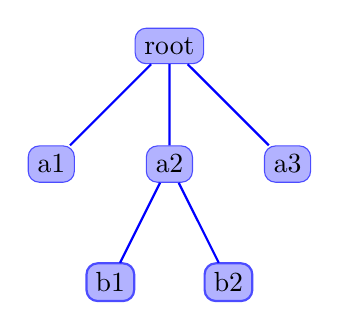
\begin{tikzpicture}
[every node/.style={fill=blue!30,draw=blue!70,rounded corners},
 edge from parent/.style={blue,thick,draw}]
    \node {root}
        child {node {a1}}
        child {node {a2}
            child {node {b1}}
            child {node {b2}}}
        child {node {a3}};
\end{tikzpicture}

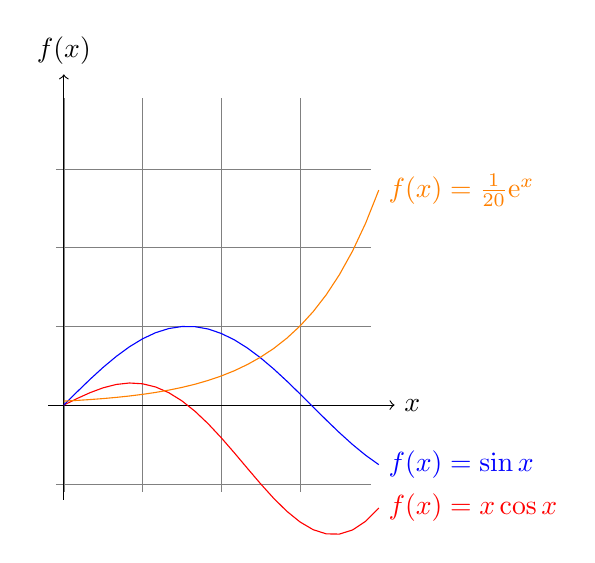
\begin{tikzpicture}[domain=0:4]
\draw[very thin,color=gray] (-0.1,-1.1) grid (3.9,3.9);
\draw[->] (-0.2,0) -- (4.2,0) node[right] {$x$};
\draw[->] (0,-1.2) -- (0,4.2) node[above] {$f(x)$};
\draw[color=red]    plot (\x,{0.5*\x*cos(\x r)})             node[right] {$f(x) =x\cos x$};
% \x r 表示弧度
\draw[color=blue]   plot (\x,{sin(\x r)})    node[right] {$f(x) = \sin x$};
\draw[color=orange] plot (\x,{0.05*exp(\x)}) node[right] {$f(x) = \frac{1}{20} \mathrm e^x$};
\end{tikzpicture}

\begin{tikzpicture}
    \graph {
        "$x_1$" -> "$x_2$"[red] -> "$x_3,x_4$";
        "$x_1$" ->[bend left] "$x_3,x_4$";
    };
\end{tikzpicture}


\chapter{一些环境}

algorithm环境
\begin{algorithm}
    \caption{Calculate $y = x^n$}
    \label{alg1}
    \begin{algorithmic}
        \REQUIRE $n \geq 0 \vee x \neq 0$
        \ENSURE $y = x^n$
        \STATE $y \leftarrow 1$
        \IF{$n < 0$}
        \STATE $X \leftarrow 1 / x$
        \STATE $N \leftarrow -n$
        \ELSE
        \STATE $X \leftarrow x$
        \STATE $N \leftarrow n$
        \ENDIF
        \WHILE{$N \neq 0$}
        \IF{$N$ is even}
        \STATE $X \leftarrow X \times X$
        \STATE $N \leftarrow N / 2$
        \ELSE[$N$ is odd]
        \STATE $y \leftarrow y \times X$
        \STATE $N \leftarrow N - 1$
        \ENDIF
        \ENDWHILE
    \end{algorithmic}
\end{algorithm}

lstlisting环境用于插入代码
\begin{lstlisting}[language=c++]
//hello.c
#include<stdio.h>
int main(void)
{
    int *p;
    printf("hello");
    return 0;
}
\end{lstlisting}

\begin{lstlisting}[language=matlab]
for i=1:100
    display('hello');
end
\end{lstlisting}

\chapter{杂项}

\begin{appendixs}
测试
\end{appendixs}

\begin{appendixs}
测试
\end{appendixs}

\begin{appendixs}
测试
\end{appendixs}

\begin{acknowledgement}
\chaptername
\end{acknowledgement}

\printbibliography[heading=bibliography,title=参考文献]
\end{document} 